\section{Processus de conception général} 
Compte tenu de la charge utile et des données de maintenance nécessaires pour la liaison descendante depuis le satellite, le spécialiste COMMS doit définir une architecture de communication avec de nombreux paramètres libres. Le processus est le suivant :

\begin{enumerate}
\item Choisissez une fréquence radio. Cette fréquence détermine la bande passante maximale disponible et dépend de la classe de la mission. De nombreuses missions CubeSat utilisent des fréquences de classe amateur ou expérimentale .

\begin{figure}[H] % H force l'affichage ici
    \centering
    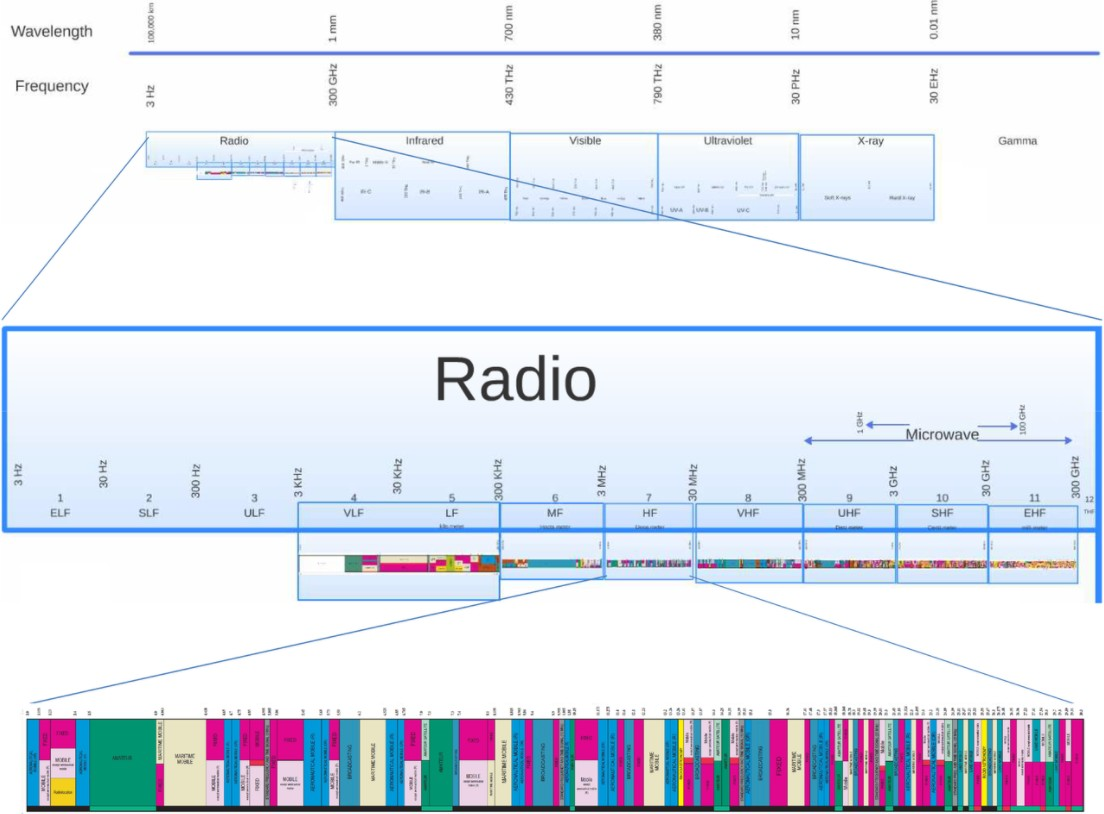
\includegraphics[width=0.5\textwidth]{figures/6-5.jpg}
    
    \caption{Haute fréquence : une vue d'ensemble de la position des hautes fréquences dans l'ensemble du spectre électromagnétique. Image d'Arkrishna.}
    \label{fig:communication2}
\end{figure}

\item Choisissez un schéma de modulation. Le schéma de modulation détermine le rapport signal/bruit requis.

\item Choisissez des algorithmes de codage qui affectent non seulement le rapport signal/bruit mais également le débit de données.
\item Analysez le temps de contact disponible que le satellite obtiendra en utilisant les stations terrestres disponibles, l'orbite et la conception de la constellation, le cas échéant. Le temps de contact est directement proportionnel à la rapidité avec laquelle le vaisseau spatial peut transmettre des données et à la fréquence à laquelle les opérateurs de mission peuvent émettre des commandes.


\end{enumerate}

Après avoir défini plusieurs options pour chaque aspect de l’architecture de communication, pour chaque alternative :

\begin{enumerate}
\item Calculer le débit de données requis à partir de toutes les sources (en fonction de l'orbite)
\item Utilisez l'équation du bilan de liaison pour dimensionner l'antenne/l'émetteur afin d'avoir une marge suffisante sur le rapport signal/bruit. Cela garantit que toutes les alternatives répondent aux exigences

\end{enumerate}
Une fois les architectures alternatives définies, utilisez d'autres mesures telles que le coût total du sous-système ou le risque pour sélectionner une alternative. Remarque : il s'agit souvent d'un processus itératif et nous pouvons modifier nos exigences en fonction de la faisabilité.
